\section{Exponential and Logarithmic Functions [WIP]}

% THIS SECTION IS

As we only need accuracy for arguments $x \in [0, 255]$, we can scale the approximation by a constant factor $\alpha$ as follows:
\begin{align*}
  \log{(1+x)} &= \log{\left(\frac{\alpha + \alpha x}{\alpha}\right)}\\
  &= \log{(\alpha + \alpha x)} - \log{\alpha}\\
  &= \log{\left(\alpha+\frac{\alpha}{n}\right)} - \log{\alpha}\\
  &= \log{\left(\frac{\alpha n + \alpha}{n}\right)} - \log{\alpha}\\
  &= \int_{n}^{\alpha n + \alpha}{\frac{1}{x}\diff x} - \log{\alpha}
\end{align*}

Applying the five-point Gauss-Legendre quadrature rule with $\alpha = 1/20$ using SageMath 8.3, we arrive at the approximation:
\begin{align}\label{eq:scaledquadrature}
  \begin{split}
    &\log(1+x) \\
    &=\frac{137x^5 + 33185x^4 + 931370x^3 - 13403630x^2 - 289469315x - 713567363}
    {30(x^5 + 505x^4 + 42010x^3 + 923010x^2 + 5722005x + 8040501)} + \log{20}
  \end{split}
\end{align}
Figure \ref{fig:scaledquadrature} is a graph of the absolute error of the scaled approximation and the exact value of $\log{(1+x)}$. Using SageMath 8.3, it was numerically determined that the maximum absolute error of this approximation in the range $x\in[0,255]$ is approximately 0.0103315865985758, occurring at $x=255$. This is an improvement from the approximation in equation \ref{eq:standardquadrature}, which has a maximum absolute error of 1.19717868468392, similarly occurring at $x=255$.

\begin{figure}[!ht]
    \centering
    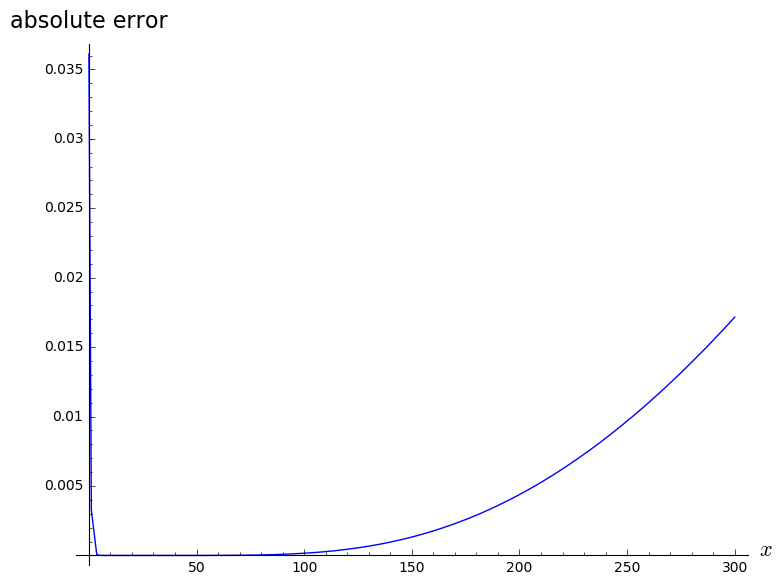
\includegraphics[width=.9\linewidth]{figures/ModifiedQuadratureAbsoluteError.png}
    \caption{Graph of the absolute error of $\log{(1+x)}$ and the approximation in equation \ref{eq:scaledquadrature}.}
    \label{fig:scaledquadrature}
\end{figure}

\subsection{Approximation for $x^\gamma$}
To approximate $x^\gamma$ for any $\gamma \in \mathbb{R}$, we rewrite $x^\gamma$ as follows:
\begin{align*}
  x^\gamma = e^{\log{x^\gamma}} = e^{\gamma\log{x}}.
\end{align*}
This expression can then be approximated using the Maclaurin series expansion for $e^x$, which converges for all $x$.
\begin{align*}
  e^x &= \sum_{n=0}^{\infty}{\frac{x^n}{n!}}\\
  \Rightarrow e^{\gamma\log{x}} &= \sum_{n=0}^{\infty}{\frac{(\gamma\log{x})^n}{n!}}
\end{align*}
As we already have an approximation for the natural logarithm, we can evaluate partial sums of the above infinite series to arrive at approximations for $x^\gamma$.
